% Assignment 2 (Mini Project): Predicting a sport game.
% NeurIPS/arXiv-style single column. Compiles under pdfLaTeX (Overleaf default), XeLaTeX or LuaLaTeX.
% Figures: python scripts/leakage_audit.py --figures-dir report/figures
\documentclass[10pt,letterpaper]{article}

\usepackage{iftex}
\ifPDFTeX\usepackage[utf8]{inputenc}\fi
\usepackage[T1]{fontenc}
\IfFileExists{newtxtext.sty}{\usepackage{newtxtext}\usepackage{newtxmath}}{\usepackage{mathptmx}}
\usepackage[scaled=0.92]{helvet}
\usepackage{courier}
\usepackage{microtype}
\usepackage[textwidth=5.5in,textheight=9in,top=1in,centering]{geometry}

\usepackage{amsmath}
\usepackage{booktabs}
\usepackage{tabularx}
\usepackage{array}
\usepackage{graphicx}
\usepackage{xcolor}
\usepackage{enumitem}
\usepackage{titlesec}
\usepackage[font=small,labelfont=bf,labelsep=period,tableposition=top]{caption}
\usepackage[colorlinks=true,allcolors={blue!60!black}]{hyperref}

% NeurIPS-like headings
\titleformat{\section}{\large\bfseries}{\thesection}{0.8em}{}
\titleformat{\subsection}{\normalsize\bfseries}{\thesubsection}{0.8em}{}
\titlespacing*{\section}{0pt}{14pt plus 2pt minus 2pt}{6pt}
\titlespacing*{\subsection}{0pt}{10pt plus 2pt minus 2pt}{4pt}
\setlength{\parskip}{0pt}
\setlength{\parindent}{15pt}
\setlist{itemsep=1pt,topsep=2pt,leftmargin=*}
\renewcommand{\arraystretch}{1.1}
\newcolumntype{Y}{>{\raggedright\arraybackslash}X}
\newcolumntype{P}[1]{>{\raggedright\arraybackslash}p{#1}}

% Float discipline: floats go to the top of a page, never force a page break.
\renewcommand{\topfraction}{0.95}
\renewcommand{\bottomfraction}{0.6}
\renewcommand{\textfraction}{0.05}
\renewcommand{\floatpagefraction}{0.85}
\setcounter{topnumber}{3}
\setcounter{totalnumber}{4}

% Visible on purpose: replace before submitting.
\newcommand{\addlink}[1]{\textcolor{red}{\textbf{[add link: #1]}}}

% NeurIPS-style abstract
\renewenvironment{abstract}{%
  \vspace{4pt}\centerline{\bfseries\large Abstract}\vspace{6pt}%
  \begin{list}{}{\leftmargin=0.5in\rightmargin=\leftmargin}\item\relax\small}
  {\end{list}\vspace{6pt}}

\title{\bfseries\Large Did My Model Predict the World Cup, or Remember It?\\[3pt]
  \large An audit of a fine-tuned LLM for football prediction}
\author{Zanwen Fu\\
  Duke University\\
  \small Assignment 2 (Mini Project): Predicting a Sport Game\thanks{The data pipeline and
  fine-tuned model were built earlier in 2026 as a separate project; this report reuses
  only their committed prediction files. Every test, baseline, figure and conclusion from
  Section~4 onward is new for this assignment, and several of them overturn claims made in
  the first version. Code and data: \url{https://github.com/zanwenfu/football-llm}. AI use
  is disclosed in Section~9.}}
\date{September 2026}

\begin{document}
\maketitle

\begin{abstract}
Earlier this year I fine-tuned Llama~3.1~8B on the 2010--2018 World Cups and reported that,
before kickoff, it called over/under~2.5 goals correctly for 76.6\% of 2022 World Cup
matches,\footnote{The first report's 76.6\% and this report's 78.1\% (Table~\ref{tab:named})
are the same model on the same prompts from two decoding runs at temperature 0.1; see
Section~4.6. I use the committed run throughout.} more than 20 points ahead of a tabular
XGBoost model, and that it turned \$1{,}000 into \$15{,}684 in a simulated backtest. For this
assignment I asked a harder question: \emph{how much of that was prediction?} Llama~3.1's
pretraining data runs to December~2023, so the 2022 results were already in the model's
weights before I fine-tuned it.

Three tests say the headline was mostly memory. Hiding the team names cuts exact-score
accuracy from 43.8\% to 10.9\%. With names shown, 59\% of predictions are the real scoreline
or its home/away mirror, against about 10\% by chance, and the tournament's famous upsets come
back with the right digits and the wrong winner. And the same backtest pays +1{,}125\% to a
rule with no model at all. Once the model cannot tell which match it is looking at, it is
statistically indistinguishable from betting ``under'' every time. What survives is that the
halftime score carries real information, but a one-line rule already captures it.

My conclusion is not that LLMs cannot predict football. It is that \textbf{accuracy on past
matches is not evidence of skill for a model that may have read the results}, and that the
test which could show skill is a forward test on matches the model has never seen, priced
against real odds.
\end{abstract}

% ---------------------------------------------------------------------------
\section{The question, and what would prove me wrong}

\paragraph{Target question.} Can a large language model predict football matches well enough
to be worth pursuing as a betting strategy?

This started in March as a fine-tuning exercise. I wanted a complete pipeline, from scraping
to a served model, on data I cared about, and World Cup matches were a good target because
the ground truth is unambiguous and the data is public. The first result looked good
(52.3\% on the winner against 45.3\% for the base model), so I kept going.

By April I had turned it into a strategy with a specific thesis. In-play bookmakers reprice
the over/under line every minute, but on coarse signals: the scoreline and the time left.
Casual in-play bettors use the scoreline and little else. The total-goals market is far
thinner than the match-winner market. So a model that has read both starting elevens'
player histories and sees the halftime score should be a better-informed participant than
most of the market, and the place to look for an edge was halftime O/U~2.5 rather than
pregame 1X2. I believed this, and I believed that more data and a bigger model would turn it
into positive returns over the long run.

The first version tested it on two decisions a bettor actually makes: who wins (1X2) and
whether the match goes over or under 2.5 goals (O/U), each made either before kickoff or at
halftime.

\paragraph{What would falsify it.} If the model has real skill, that skill should not depend on
it knowing \emph{which} match it is predicting. If its advantage disappears once it cannot
identify the match, then what I measured was recall of results it had read, not prediction.
I built this control when I built the model (a copy of every test prompt with the team names
replaced by ``Team~A'' and ``Team~B''), saw the model do slightly \emph{better} with names
hidden on the winner (54.7\% vs.\ 50.0\%), and wrote that this was the single most important
validation result for the strategy. Section~4 shows I read it on the wrong metric.

% ---------------------------------------------------------------------------
\section{Analytical framework}

Following the research process from Lecture~5, I sampled the questions that different roles
would ask of this project,\footnote{Prompt used, once per role: ``You are a
\emph{[bettor / match analyst / sports statistician / ML evaluator]}. For a project that
predicts World Cup match scores with a fine-tuned language model, list the key question you
would ask, the measure that answers it, and the data that measure needs. No computation.''}
and then checked which of their measures my data can support.

\begin{table}[t]
\small
\caption{Roles, key questions, measures, and data availability.}
\label{tab:roles}
\begin{tabularx}{\textwidth}{@{}P{2.5cm}YYP{3.8cm}@{}}
\toprule
Role & Key question & Measure & Available to me? \\
\midrule
Bettor / trader & Does the model beat the price after the bookmaker's cut? &
  Return against real odds; break-even hit rate (52.6\% at odds 1.90) &
  \textbf{No odds data.} My earlier backtest assumed 1.90 on every match. \\
Match analyst & Who is stronger, and what is the game state? &
  Starting XI's prior-season player stats; halftime score &
  Yes (API-Football) \\
Sports statistician & How many goals should each side score? &
  Dixon-Coles expected goals $\lambda,\mu$; O/U probability &
  Only World Cup results (256 matches) \\
ML evaluator & Is the measured skill real, or leaked? &
  Named vs.\ hidden gap; mirror test; trivial baselines; power &
  Yes (built for this audit) \\
\bottomrule
\end{tabularx}
\end{table}

Lecture~7 ranks the data types that decide soccer predictions. Setting my inputs against
that ranking was sobering (Table~\ref{tab:datatypes}): the model saw only the fifth-ranked
type and none of the top four.

\begin{table}[t]
\small
\caption{The model's inputs against the lecture's ranking of predictive data types.}
\label{tab:datatypes}
\begin{tabularx}{\textwidth}{@{}rP{5.2cm}Y@{}}
\toprule
Rank & Data type (Lecture 7) & In my model's input? \\
\midrule
1 & Historical match outcomes & Only World Cup matches, 3--7 per team every four years \\
2 & Betting-market probabilities & None \\
3 & Team strength ratings (Elo, etc.) & None \\
4 & Team performance statistics (xG, form) & None (StatsBomb xG exists for 2018/2022 only; unused) \\
5 & Player statistics \& availability & \textbf{Yes: the only real input} \\
8 & Match context (venue, stage) & Yes, which turns out to matter for leakage (Section~4.3) \\
\bottomrule
\end{tabularx}
\end{table}

% ---------------------------------------------------------------------------
\section{What I built, and what I claimed}

\paragraph{Pipeline.} From API-Football I scraped all 256 World Cup matches from 2010 to 2022
(results, halftime scores, lineups, events) and about 168{,}000 rows of player statistics
(one per player, season and competition) from 2004 to 2025. For each match, the starting XI's
statistics from the three seasons \emph{before} the tournament are aggregated into a short
text profile per team. Llama~3.1~8B Instruct was fine-tuned with QLoRA on the 192 matches of
2010, 2014 and 2018 to answer \texttt{Prediction / Score / Reasoning}, and tested on the 64
matches of 2022, each shown twice: with team names, and with names hidden.

\paragraph{Models compared in this audit} (all on the same 64 matches):
the LLM with team names; the LLM with names hidden; XGBoost trained on the same features;
a Dixon-Coles model fitted to 2010--2018 results (new, following Lecture~7); and rules that
use no model (``always under'', ``double the halftime goals'').

\paragraph{What I first claimed.} LLM and XGBoost tied on 1X2, but the LLM won on goals:
39.1\% vs.\ 6.2\% exact scores and 76.6\% vs.\ 54.7\% on O/U before kickoff. I attributed
this to ``pretrained scoreline priors'' and called it a magnitude/direction decomposition. I
also reported that halftime conditioning lifted 1X2 accuracy with $p=0.024$, that adding
first-half events raised O/U accuracy to 79.7\%, and a simulated return of +1{,}468\%.
Several of those numbers do not survive the audit, and one cannot be regenerated at all
(Section~4.5).

% ---------------------------------------------------------------------------
\section{The audit}

Lecture~6 gives a seven-item validation checklist. I worked through it in the order that
turned out to matter.

\subsection{Out-of-sample test: the test set was not out of sample}

Llama~3.1 was released in July~2024 with pretraining data through December~2023. The 2022
World Cup, including every score, was on the public web the model was trained on. My split
was clean for the \emph{fine-tuning} data (2010--2018 in, 2022 out) and for the features
(only seasons before each tournament), but not for the \emph{base model}. This is exactly the
failure in Lecture~7's W-5 case: ``training data holds post-event knowledge'', and ``pretend
not to know'' does not work because the knowledge is in the parameters.

\subsection{Cross-validation with outcomes: hide the names}

\begin{table}[t]
\small
\caption{Accuracy (\%) with and without team names. The model is identical; only the names differ.}
\label{tab:named}
\begin{tabularx}{\textwidth}{@{}Y rrr r rrr@{}}
\toprule
& \multicolumn{3}{c}{Pregame} & & \multicolumn{3}{c}{Halftime} \\
\cmidrule{2-4}\cmidrule{6-8}
64 matches, same prompts except names & 1X2 & Exact & O/U 2.5 & & 1X2 & Exact & O/U 2.5 \\
\midrule
LLM, team names  & 50.0 & 43.8 & 78.1 & & 64.1 & 51.6 & 81.2 \\
LLM, names hidden & 53.1 & 10.9 & 56.2 & & 64.1 & 18.8 & 70.3 \\
\addlinespace
Paired McNemar $p$ (names vs.\ hidden) & 0.82 & $<$0.001 & 0.007 & & 1.00 & $<$0.001 & 0.12 \\
\bottomrule
\end{tabularx}
\end{table}

Knowing the names does not help the model pick the winner at all (50.0\% vs.\ 53.1\%), but it
quadruples exact scores. My original notebook compared the two versions on 1X2 only, saw no
gap, and concluded the model ``learned from stats, not names''. \textbf{I had the right
control and read it on the one metric where memory helps least.} A model that remembers
``it finished 1--0'' but not who won is exactly what this table looks like.

\subsection{Model interpretation: the mirror test}

If the model half-remembers a result, it should often reproduce the scoreline's digits but
not always their order. I counted predictions that match the real score exactly \emph{or}
with home and away swapped, and compared that rate with a null in which each model's own
predictions are matched to shuffled fixtures. The null keeps both the model's score
distribution and the tournament's, so it already credits common scores like 1--0.

\begin{figure}[t]
\centering
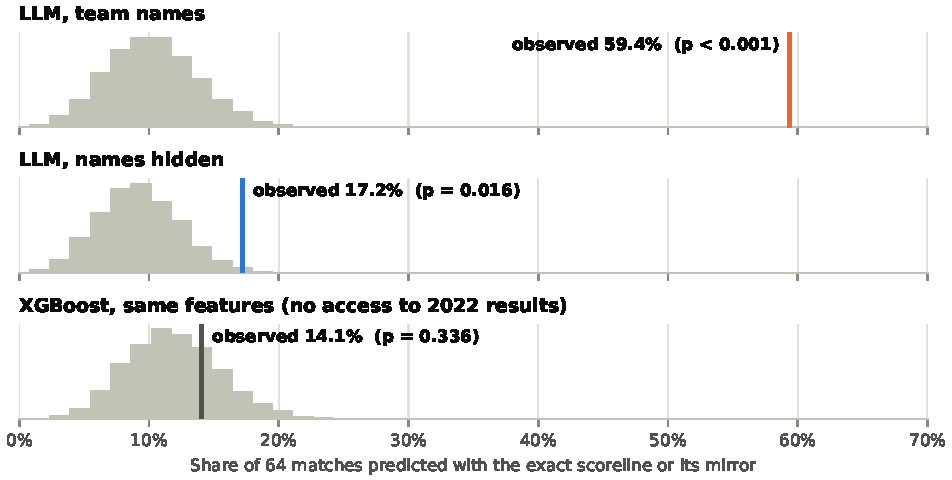
\includegraphics[width=\textwidth]{figures/fig_mirror_test.pdf}
\caption{Exact-or-mirrored scorelines, pregame. Gray: 10{,}000 shuffles of each model's own
predictions. XGBoost, which has no route to the 2022 results, sits inside its null.}
\label{fig:mirror}
\end{figure}

With names, 59.4\% of predictions are the real score or its mirror ($p<0.001$). The ten
mirrored cases are telling: \emph{Tunisia 1--0 France} was predicted 0--1, \emph{Morocco 1--0
Portugal} 0--1, \emph{Japan 2--1 Germany} as Germany 2--1, \emph{Qatar 0--2 Ecuador} 2--0. The
model recalls the scoreline and assigns the win to the stronger team on paper. It also
predicted correctly scores no statistics could produce, such as England 6--2 Iran, Portugal
6--1 Switzerland, and 3--3 for the final, which is the score \emph{after extra time}. This
single mechanism explains the ``magnitude/direction decomposition'' I reported in the first
version: it is the signature of memory, not a scoreline prior.

The hidden-name model also beats its null ($p=0.016$) while XGBoost on the same features does
not ($p=0.34$). The hidden prompts still contain the coach's name, the stadium and the round
(``Team~A | Coach: G.~Southgate'', ``Group Stage -- 1 | Al Bayt Stadium''), which together
identify the match. The evidence is weak at $n=64$, but it means even my ``names hidden''
numbers are an upper bound.

\subsection{Cross-validation with benchmarks}

\begin{figure}[t]
\centering
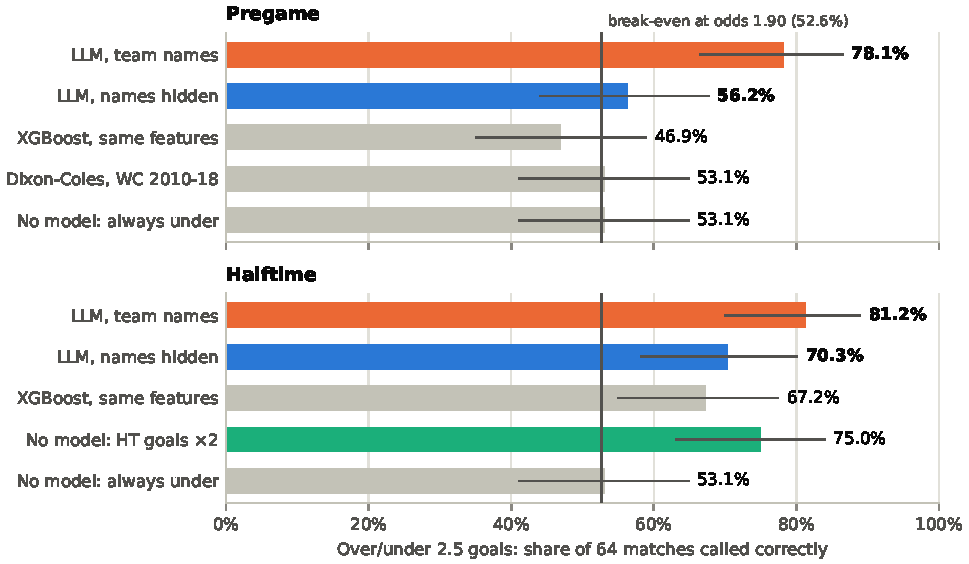
\includegraphics[width=\textwidth]{figures/fig_ou_accuracy.pdf}
\caption{O/U~2.5 accuracy on the same 64 matches, with 95\% Wilson intervals. The vertical
line is the hit rate needed to break even at odds of 1.90.}
\label{fig:ou}
\end{figure}

\begin{table}[t]
\small
\caption{Every model on the same matches (\%). With names hidden, nothing clearly beats a constant.}
\label{tab:benchmarks}
\begin{tabularx}{\textwidth}{@{}Y rrr r rr@{}}
\toprule
& \multicolumn{3}{c}{Pregame} & & \multicolumn{2}{c}{Halftime} \\
\cmidrule{2-4}\cmidrule{6-7}
Model (64 matches) & 1X2 & Exact & O/U & & 1X2 & O/U \\
\midrule
LLM, names hidden & 53.1 & 10.9 & 56.2 & & 64.1 & 70.3 \\
XGBoost, same features & 57.8 & 12.5 & 46.9 & & 62.5 & 67.2 \\
Dixon-Coles, fitted on WC 2010--2018 & 45.3 & 7.8 & 53.1 & & -- & -- \\
No model: always home win / always under & 45.3 & -- & 53.1 & & 45.3 & 53.1 \\
No model: halftime leader wins / halftime goals $\times2$ & -- & -- & -- & & 56.2 & \textbf{75.0} \\
\bottomrule
\end{tabularx}
\end{table}

Pregame, with the names hidden, the LLM's 56.2\% on O/U is within noise of ``always under''
(53.1\%); XGBoost is worse than that constant. At halftime, simply doubling the first-half
goals gets 75.0\%, ahead of the hidden-name LLM's 70.3\% (paired $p=0.66$).

The Dixon-Coles model from Lecture~7 taught me something on its own. I chose its shrinkage
by fitting on 2010--2014 and scoring 2018, never looking at 2022, and the best out-of-sample
setting was maximum shrinkage: every team average. Team strengths from one World Cup barely
transfer to the next, because each team plays three to seven matches every four years. With
this data the textbook benchmark collapses to a constant, which is Lecture~7's own warning
(``Not yet, the current model is overfitting with the data set!'') and says the real
bottleneck is data type~1 in Table~\ref{tab:datatypes}.

One limit of the comparison: the LLM outputs a scoreline, not a probability, so I cannot
report Brier or log loss for it as Lecture~7 does for W-5. Turning a predicted score into
$P(\text{over}~2.5)$ needs a Poisson step, which is a second model. Dixon-Coles gives
probabilities directly (O/U Brier 0.250, no better than a coin), and the forward test in
Section~7 will need the LLM to do the same, by sampling several completions per match.

\subsection{Data validation}

\begin{itemize}
\item \textbf{A result I cannot reproduce.} The first version's third regime (halftime plus
  first-half events: 79.7\% O/U, calibration error 0.182, $p=0.006$) came from a scratch run
  whose predictions were never saved. I drop those numbers.
\item \textbf{Labels include extra time.} Bets settle at 90 minutes, but my labels use the
  final score (Argentina--France is labelled 3--3; it was 2--2 at 90 minutes). This affects
  2 test and 9 training matches. The Dixon-Coles model trains on 90-minute scores.
\item \textbf{The hidden prompts are only partly hidden} (coach, stadium, round; above).
\end{itemize}

\subsection{Stability}

\begin{itemize}
\item \textbf{Two runs, two answers.} Inference sampled at temperature 0.1. Two runs of the
  same weights on the same prompts gave 52.3\% and 51.6\% 1X2 accuracy, and my earlier README
  mixed numbers from both.
\item \textbf{Double counting.} My earlier $p=0.024$ for the halftime lift pooled the named
  and hidden copies ($n=128$), counting every match twice. Tested within each copy ($n=64$),
  the lift is $p=0.049$ with names and $p=0.21$ without.
\item \textbf{Width of the evidence.} At $n=64$ a 95\% interval on an accuracy is about
  $\pm$12 points wide, so most model-to-model differences here are not resolvable.
\end{itemize}

\subsection{Error analysis}

The outputs have problems that are about decoding, not modelling. Before kickoff the model
predicted 1 draw in 64 matches with names and 0 without, against 15 real draws. It also
produced 9 (names) and 11 (hidden) scorelines with one side on six or more goals, such as
0--8, 2--8 and 6--8, against 3 real ones. And in 24 of 64 pregame outputs its written label
contradicts its own score. Inference used a repetition penalty of 1.1, which discourages
repeating a digit and may be why 0--0 and 1--1 come out as 0--8 and 1--6. I have not verified
this, since it needs a GPU rerun.

\subsection{Backtest and forward test}

\begin{figure}[t]
\centering
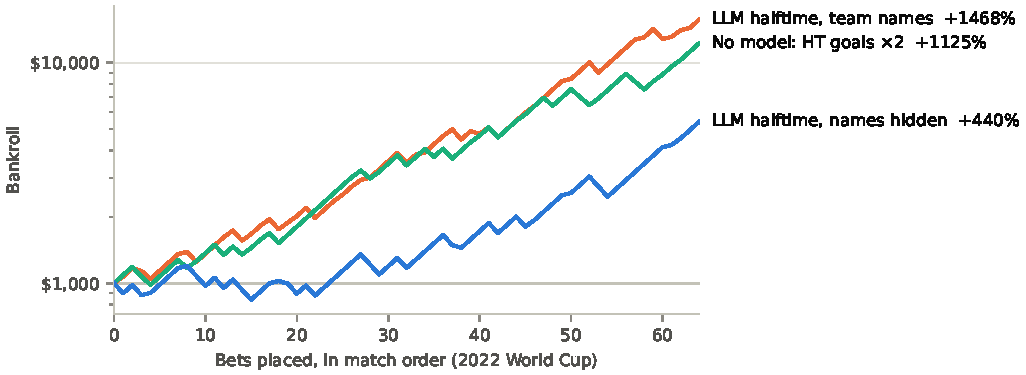
\includegraphics[width=\textwidth]{figures/fig_flat_odds_backtest.pdf}
\caption{My original backtest (O/U~2.5 at odds 1.90 on every match, quarter Kelly, 10\% cap),
run on three strategies. Log scale; \$1{,}000 start.}
\label{fig:backtest}
\end{figure}

The original simulation assumed odds of 1.90 on both sides of every match. At halftime that
assumption hands an edge to anyone who can see the score, because a real bookmaker reprices
the line when it is 2--0 at the break. The proof is Figure~\ref{fig:backtest}: \textbf{a rule
with no model returns +1{,}125\%}. The hidden-name LLM returns +440\% at halftime and
$-0.4$\% before kickoff. The simulation was measuring memory and its own odds assumption,
not skill.

Even with real odds, one tournament cannot establish an edge. With flat stakes at odds
1.90, detecting a true edge of 5\% per bet (one-sided $\alpha=0.05$, power 0.8) takes about
2{,}200 bets; 2\% takes about 13{,}900. A World Cup has 64 matches, 104 from 2026.

% ---------------------------------------------------------------------------
\section{What survives}

\begin{itemize}
\item \textbf{The halftime score is real information.} With names hidden, halftime
  conditioning moves O/U from 56.2\% to 70.3\% and 1X2 from 53.1\% to 64.1\%, though neither is
  significant at $n=64$ ($p=0.09$, $p=0.21$). The model generalises to a prompt field it was
  never trained on. But a one-line rule captures the same information at least as well.
\item \textbf{Before kickoff, I find no skill} once the model cannot identify the match.
\item \textbf{The infrastructure is sound and reusable:} temporal feature windows, the
  named/hidden control, and now an audit that runs in one second and flags leakage
  automatically. That is what makes the forward test in Section~7 cheap.
\end{itemize}

% ---------------------------------------------------------------------------
\section{What I believe now}

\paragraph{Then.} a model that has read the players' histories and sees the halftime score is
better informed than the in-play market, and with more data and a bigger model that edge
would compound.

\paragraph{Now.} I had the wrong bottleneck. I spent months on the model and almost no time on
the test, and the test is where the project failed. Five things changed my mind.

\begin{enumerate}
\item \textbf{I read my own control until it passed.} The names-hidden test was the right
  idea. On the winner it showed no gap, so I stopped looking and called it clean. On the
  score, which is what my whole O/U thesis rested on, names quadrupled accuracy. I wanted
  the control to pass and I checked it on the one metric where memory helps least. That is
  the part of this project I am least comfortable with, and it is why every number in this
  report is printed by a script rather than copied from a notebook.
\item \textbf{The halftime edge I was excited about is mostly the halftime score.} Doubling
  first-half goals beats my model at halftime. My thesis was that the market ignores
  player-level information once the score is known. I never tested that, because I never
  had the market's price. What I tested was whether a model with the score beats a model
  without it. That is not an edge over anyone.
\item \textbf{A stronger model would make this backtest look better for the wrong reason.}
  A newer, larger LLM has read more results. On any test set before its training cutoff it
  scores higher by remembering more. Scaling the model makes the measurement worse unless
  the test is on matches it cannot have seen.
\item \textbf{Capacity cannot create information that is not in the input.} My prompts
  held data type~5 and none of types 1--4 in Table~\ref{tab:datatypes}. A bigger model
  reads the same player totals.
\item \textbf{Returns come from beating prices, and World Cups are too small to show it.}
  A 56\% hit rate is only worth something against a price that implies less, and I never
  compared to a real price. Proving even a 5\% edge takes about 2{,}200 bets. That means
  club leagues, where the market is most efficient, not one tournament every four years.
\end{enumerate}

I still think the idea is worth testing, in narrower forms: an LLM as a reader of
unstructured information the market prices slowly (team news, injuries, confirmed lineups),
especially in thinner markets, or as a feature extractor feeding a calibrated model such as
Dixon-Coles rather than as the predictor itself. \textbf{What would change my mind back} is
a pre-registered forward test on matches after the model's training cutoff, with identities
properly hidden, that beats closing odds by more than the bookmaker's margin over hundreds
of bets. Until then, the honest summary of the first version is that it built a good
pipeline and measured the wrong thing.

% ---------------------------------------------------------------------------
\section{Plan for the final project}

\begin{table}[t]
\small
\caption{From Assignment~2 to the final project.}
\begin{tabularx}{\textwidth}{@{}P{5.2cm}Y@{}}
\toprule
Gap found in this audit & Fix \\
\midrule
Test set inside the base model's training data &
  Forward test on matches after December 2023: Euro 2024 and Copa Am\'erica 2024 (about 83
  matches) and the 2026 World Cup (104 matches) \\
Hidden prompts leak via coach, stadium, round & Strip them; confirm with the mirror test \\
No market benchmark & Collect closing odds; report return and closing-line value \\
Sparse history & All international results for Dixon-Coles and Elo benchmarks \\
Decoding problems & No repetition penalty, deterministic decoding, several samples per match for probabilities \\
Extra-time labels & Train and score on 90-minute results \\
Halftime prompts never trained on & Fine-tune on halftime prompts; compare against the halftime rule \\
\bottomrule
\end{tabularx}
\end{table}

% ---------------------------------------------------------------------------
\section{Reproducing every number}

No GPU is needed; everything runs in seconds from the committed prediction files.
{\small\begin{verbatim}
pip install -e ".[dev]"
python scripts/leakage_audit.py --figures-dir report/figures
python -m football_llm.baselines.dixon_coles
python scripts/reproduce_paper.py --skip-figures
\end{verbatim}}
The first script prints every number in Sections~4 and~5 and writes the figures; the second
fits and scores the Dixon-Coles benchmark; the third regenerates the original tables.

% ---------------------------------------------------------------------------
\section{AI use disclosure}

I used AI assistants throughout and am disclosing all of it as the assignment requires.

\paragraph{Building the model (earlier in 2026).} The data pipeline, training, evaluation and
serving code, and the first write-up and README, were written with heavy AI assistance
(Claude and GitHub Copilot), with me directing, debugging and running everything.

\paragraph{This assignment.} What I did: chose to audit the project rather than extend it,
answered the questions about what I believed in March and April and why, decided which
tests to run, reviewed every section and table against the script output, and wrote
Sections~1 and~6 in my own words. What Claude (Anthropic) did: in the first dialogue below it
read the repository, flagged that the 2022 test set sits inside Llama~3.1's pretraining data,
and proposed the named-versus-hidden split and the trivial baselines. In a Claude Code
session it wrote \texttt{scripts/leakage\_audit.py}, \texttt{dixon\_coles.py} and their tests,
ran the analyses, and drafted the remaining sections and the updated README, which I edited.
Every number in this report is printed by the scripts in Section~8.

Dialogues:
\begin{itemize}
\item Claude conversation reviewing the project and identifying the gaps: \addlink{first chat}
\item Claude Code session that built the audit and drafted this report: \addlink{Claude Code session}
\end{itemize}

\end{document}